% We do not want to have screen shots of the celebrity puzzle in this section:
\clearpage
\section{Location Access Controller}
\label{tut_location_access_controller}

\tick{\textbf{Goals:} In this section, we will take a closer look at a few more complex proofs. For this we use the model of a location access controller. The goal is to develop the proofs that ensure there are no deadlocks present in the initial model and in the first refinement.}

%\info {First of all you need to download the following \file{Doors.zip}{Location Access Controller problem}.}

Through the model used in this section, we study a complete system and remind the proof rules of formal development. The system's task is to control the access of certain people to different locations of a site. The system is thus based on whether a person has (or does not have) access to a particular location.

Before describing the initial model, import the archive file \file{Doors.zip}{Doors.zip} that contains the model. To do this, select  \textsf{File $\rangle$ Import $\rangle$ General $\rangle$ Existing Project into Workspace}. Then select the according archive file and click on \textsf{Finish}. It will take Rodin a few seconds to extract and load all the files.

\subsection{Initial Model} 
\label{tut_initial_model}

%Besides we introduce:

%\begin{itemize}
%	\item The two carrier sets of persons, P, and locations, L
%	\item The constant authorization, \textbf{aut}, representing a relation between P and L, actually where people are allowed to go %(Axiom 1).
%	\item The variable, \textbf{sit}, which denote where a person is, \textbf{sit} is a function from P to L.
%\end{itemize} 
 
%Moreover, we introduce a special constant “location”, named \textbf{outside}. Everyone is authorized to be in outside (Axiom 3) and a %person cannot be in two locations at a time. However every person, which is in a certain location, is authorized to be there.

%Initially, everyone is outside as indicated in event \textsf{INITIALISATION}.
%The other event \textsf{PASS} of that model has to aim to change the location of a person.
%We call the proof of deadlock freeness through this tutorial the proof justifying that someone can always change location.

Let us look at the initial model which consists of \texttt{doors\_ctx1} and \texttt{doors\_0}. There are two carrier sets in the model context. One is for people (\textsf{P}) and the other is for locations (\textsf{L}). There is a location called outside (\textsf{outside}) and a relation (\textsf{aut}) which reflects where people are allowed to go. Everyone is permitted to go \textsf{outside}. The model machine has one event, \textsf{pass}, which changes the location of a person and one variable, \textsf{sit}, which denotes where a person is located. 

\subsubsection{Deadlock Freeness}
\label{deadlock}

Looking through the initial model, you will see that everything already has been proved. This is true, but Rodin does not do any deadlock freeness proof yet, so we will have to add them by ourself. A model is considered as deadlocked if the system reaches a state with no outgoing transitions. The objective of this section is to develop proofs for deadlock freeness for the initial model and for the first refinement. 

Consider the event \textsf{pass} from the initial model:

\begin{description}
\EVENTS
	\EVT {pass}
		\begin{description}
		\AnyPrm
			\begin{description}
			\ItemX{ p }
			\ItemX{ l }
			\end{description}
		\WhereGrd
			\begin{description}
			\nItemX{ grd11 }{ p \mapsto  l \in  aut }
			\nItemX{ grd12 }{ sit(p) \neq  l }
			\end{description}
		\ThenAct
			\begin{description}
			\nItemX{ act11 }{ sit(p) :=  l }
			\end{description}
		\EndAct
		\end{description}
\END
\end{description}

\index{deadlock}
Since the initial model has only one event (\textsf{pass}), the system might deadlock when both guards of the event (\textsf{grd11} and \textsf{grd12}) are false. In this case, to prove that no deadlocks can occur requires proving that someone can always change room. Clearly, we want to avoid this happening. We must therefore prove that the two guards are always true. To do this, add a new derived invariant (a theorem) to \texttt{doors\_0} called \textsf{DLF} (click the \texttt{not theorem} button to make it switch to \texttt{theorem}) and change the predicate so that it is the conjunction of the two guards.
The difference between a ``normal'' invariant and one that is marked as theorem is that is must be proven that the theorem always holds if the other invariants declared before hold. We do not need to prove that an event preserves the invariant marked as theorem because this is a logical consequence when it preserves the other invariants.

\begin{description}
\INVARIANTS
	\begin{description}
		\nItemX{ DLF }{ \exists p, l\qdot (p \mapsto  l \in  aut \land  sit(p) \neq  l) }
	\end{description}
\end{description}


\begin{rodin-plugin}{img/prob.png}{ProB}%
  You can also use ProB to search for deadlocks.
  Right-click on the machine you want to check and start the animation with the
  ``Start Animation / Model Checking'' menu entry.
  After starting the animation, go to the Event View in the ProB perspective
  (see \ref{fig_tut_prob_perspective}).
  There are two ways to search for deadlocks:
  \begin{itemize}
  \item Just press on the \texttt{Check} button and mark \texttt{Find Deadlocks} before
    starting the check by pressing the button \texttt{Start consistency checking}.
    ProB then systematically ``executes'' all events and tries to find a state where no
    event is enabled.
  \item An alternative is to select \texttt{Deadlock Freedom Checking} after clicking
    on the triangle right to the \texttt{Check} button.
    ProB then prompts you for an optional predicate. Just leave that empty for the start.
    The difference to the first alternative is that ProB searches now for variable values
    where all invariants are true but none of the guards.
  \end{itemize}
\end{rodin-plugin}

Save the machine. We will see in the Event-B Explorer View that the autoprover (\ref{auto_prover}) fails to prove the theorem \textsf{DLF/THM}.

\warning{If you cannot find the proof obligation \textsf{DLF/THM}, maybe you forgot to mark the invariant as a theorem by clicking on the \texttt{theorem} button. Another reason that you don't see the proof obligation \textsf{DLF/THM} could be that you forgot to rename the invariant ``DLF''.}

Let us analyze whether this is an inconsistency in the model. Switch to the \texttt{Proving Perspective } and double click on the proof obligation \textsf{DLF/THM}.

%\begin{center}
%	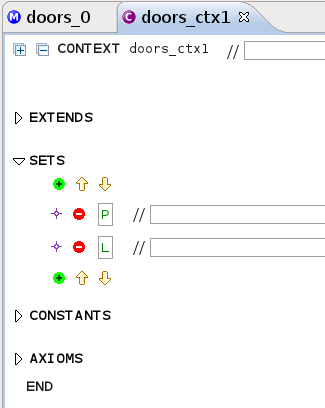
\includegraphics[]{img/tutorial/tut_10_carrier-sets.png}
%\end{center}

%\begin{center}
%	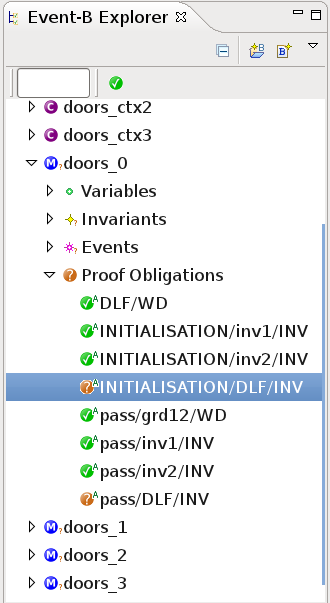
\includegraphics[]{img/tutorial/tut_10_proversfailed.png}
%\end{center}

In order to succeed with the proof, we need a tuple $p \mapsto l$ that is in \textsf{aut} but not in \textsf{sit}. Searching the hypotheses, we find the \textsf{axm4} of \texttt{doors\_ctx1}, which states that there is a location \textsf{l} where everyone is allowed to go:

\begin{description}
\AXIOMS
	\begin{description}
		\nItemX{ axm4 }{ \exists l\qdot l\in L\setminus \{ outside\}  \land  P\cprod \{ l\} \subseteq aut }
	\end{description}
\end{description}

So for every person \textsf{p} in \textsf{P}, $p \mapsto l$ and $p \mapsto outside$ are in \textbf{aut}. Since these are different, at least one of them cannot be in the function \textbf{sit}. All we need to prove now is that \textsf{P} is nonempty. This holds since carrier sets are always nonempty, but is a bit hard to prove. 

\warning{In the Proof Control view, first disable the post-tactics (there is a small downward pointing arrow in the upper right hand corner above the toolbar, see Figure~\ref{fig_tut_10_post_tactics}. Click on this arrow and make sure that the option \textsf{Enable post-tactic} is unchecked in the dropdown menu. We turn off the post-tactics because we want to see the proof develop in its different stages.)}

\begin{figure}[!ht]
  \begin{center}
    	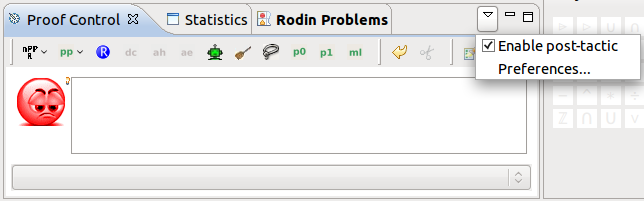
\includegraphics{img/tutorial/tut_10_post_tactics.png}
    \caption{Disabling the proof post-tactics in the Proof Controling View}
    \label{fig_tut_10_post_tactics}
  \end{center}
\end{figure}

%\begin{center}
%	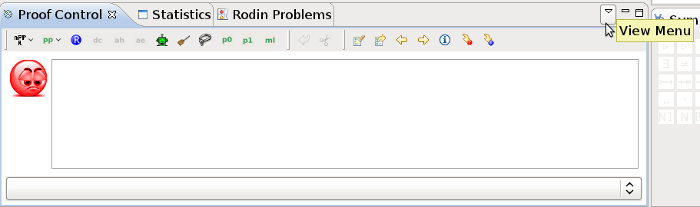
\includegraphics[]{img/tutorial/tut_10_view_menu.png}
%\end{center}

Now add the hypothesis $\exists x . x \in P$ using the \icon{rodin/ah_prover.png} button after entering the predicate into the Proof Control text area. 
In the \textsf{Proof Tree} view you can now see three new nodes, $\btrue$, $\exists x\qdot x\in P$ and the original goal.
Click on the \icon{rodin/auto_prover.png} button to prove $\btrue$, the well-definedness condition
of our hypothesis. Then click \icon{rodin/auto_prover.png} another time to prove the hypothesis itself. Other provers do not work here. The first two of the three nodes are now marked as proven. After successfully adding the hypothesis, we can conclude the proof as follows:

Click on the existential quantifier of the expression $\exists x \cdot x \in P$ (appearing in the \textsf{Selected Hypothesis} view) as demonstrated in Figure \ref{fig_tut_10_instantiate_x}. You see that it is automatically instantiated. It leads to the selected hypothesis $x \in P$. We can now instantiate \textsf{p} in the goal with \textsf{x}: enter \textsf{x} in the yellow box corresponding to \textsf{p} in the \textsf{Goal View} and click on the existential quantifier as shown in Figure \ref{fig_tut_10_instantiate_p}. 

\begin{figure}[!ht]
\begin{center}
	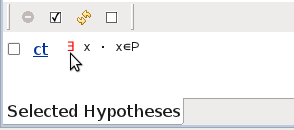
\includegraphics{img/tutorial/tut_10_instantiate_x.png}
	\caption{Click on the existential quantifier in order to ...}
	\label{fig_tut_10_instantiate_x}
\end{center}
\end{figure}

\begin{figure}[!ht]
\begin{center}
	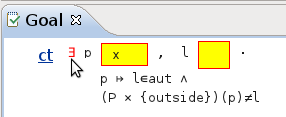
\includegraphics{img/tutorial/tut_10_instantiate_p.png}
	\caption{... instantiate it, in this case by substituting $x$.}
	\label{fig_tut_10_instantiate_p}
\end{center}
\end{figure}

\warning{If the hypothesis does not appear immediately in the \textsf{Selected Hypothesis} view, reclick on the Auto Prover button until it does.}

Now \textsf{l} needs to be instantiated. In order to instantiate it, we need a case distinction. Type sit(x) = l into the \textsf{Proof Control View} and click on \textsf{Case Distinction button (dc)} to look at the two cases $sit(x) = l$ and $sit(x) \neq l$. Before starting with the cases, the prover now wants you to prove that $x \in dom(sit)$. This can be done with the \textsf{p0} prover since \textsf{sit} is a total function (\ref{relations}). In the first case, \textsf{x} is situated in \textsf{l}, so it cannot be in \textsf{outside}. You can instantiate \textsf{l} with \textsf{outside} (type \textsf{outside} in the box corresponding to \textsf{l} and click on the existential quantifier). In order to prove that \textsf{x} is allowed \textsf{outside}, you will need to select the hypothesis $P \times {outside} \subseteq aut$ (if this hypothesis doesn't appear in the search hypothesis, type outside in the proof control view, click on the \textsf{Search Hypothesis button} and add it to the selected hypothesis using the green plus icon). Then you can finish this case with the \textsf{p0} prover (select the items from this case from the proof tree and hit the \textsf{p0} button. If this doesn't work, hit the \icon{rodin/lasoo_prover.png} button to select all of the necessary hypotheses and try again). Now you have reached the other branch of the case distinction in the proof tree. In this case, you can simply instantiate \textsf{l} with \textsf{l} since 
\textsf{x} is not situated there. Finally, use the \textsf{p0} button to finish the proof. 

\subsection{First Refinement}
\label{tut_location_first_refinement}

Now we are going to explain the main complexity of our model: the deadlock freeness proof for the first refinement. 

The difference between the first refinement and the initial model is that a new constant \textsf{com} been added in order to describe which rooms are connected. Additionally, we have a constant \textsf{exit}, which will be explained later. 

The event \textsf{INITIALISATION} does not change, but the event \textsf{PASS} is refined as a consequence. We assume that a person can move to another location l if they have the authorization to be in l (already defined in the abstraction) and also if the location l is connected to the location p where the person is at this precise moment (represented by sit(p)).

We need to add a new guard that is more exact that that of the machine it refines:

\[
( sit(p) \mapsto l \in com ) \Rightarrow ( sit(p)\neq l )
\]

We are faced with a difficulty here; it is not possible to prove that the refined event \textsf{PASS} does not happen less often than the abstract event \textsf{PASS} of its predecessor. To prove this we would have to prove that the guard of the abstract event implies that of the concrete event.

The issue is that this condition cannot be verified in general. Moreover, the failure to prove the above condition indicates that there are possibilities that certain people could stay permanently blocked in locations. People are also more limited in the ways that they may move because they can only move between rooms that are connected.

Now we know that this model contains a problem ignored in the document requrements. We must now find a sufficient solution.

\info{Please note that post-tactics should still be disabled before starting this part of the tutorial.} 

At the beginning of this section we need to come back to the \textsf{Event-B Perspective}. As described in Section \ref{tut_initial_model}, open \texttt{door\_1} machine and add a derived invariant (theorem) called \textsf{DLF} as follows: 

\begin{description}
\INVARIANTS
	\begin{description}
		\nItemX{ DLF }{ \exists q, m \cdot (q \mapsto m \in aut \wedge sit(q) \mapsto m \in com)  }
	\end{description}
\end{description}

Save the file. Once again, the prover fails to prove the deadlock freeness automatically. Actually all we want to prove is that ``any person authorized to be in a location must also be authorized to go in another location which communicates with the first one''.

This can be illustrated as demonstrated in Figure \ref{fig_tut_10_graph}.

\begin{figure}[!ht]
\begin{center}
	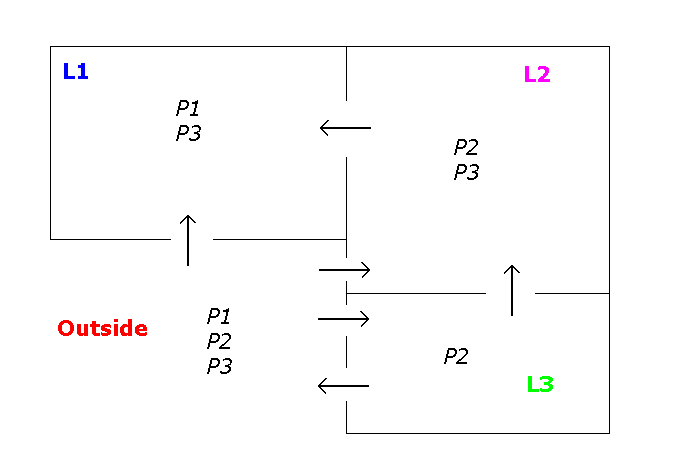
\includegraphics[]{img/tutorial/tut_10_graph.png}
	\caption{The floorplan of the location to be controlled.}
	\label{fig_tut_10_graph}
\end{center}
\end{figure}

To begin with, switch over to the proving perspective and double click on \textsf{DLF/THM} to begin proving. At the beginning of the proof, there aren't any selected hypothesis, so we need to select a few. The old deadlock freeness invariant will be useful, and \textsf{axm7} of \texttt{doors\_ctx2} as well. 

\begin{description}
\AXIOMS
	\begin{description}
		\nItemX{ axm7 }{ \exists l\qdot l\in L\setminus \{ outside\}  \land  outside\mapsto l\in com \land  P\cprod \{ l\} \subseteq aut  }
	\end{description}
\end{description}

We will try to avoid using \textsf{exit} since we want to keep things as simple as possible. Because \textsf{sit} and \textsf{aut} are inside the invariant, we also are likely to need 

\[
sit \subseteq aut \land sit \in P \mathbin \rightarrow L.
\]

Once again, the prover automatically rewrites the existential quantifiers in the hypotheses. We now look at the proof. There is an easy case if $sit(p) = outside$. Add this case as previously using the \textsf{Case Distinction button (dc)}. To do this, you first need to instantiate the value for p. To do this, use the hypothesis $\exists p, l \cdot p \mapsto l \in aut \land sit(p) \neq l$ and then click on the existential quantifier to create the expression $ p \in P $ (see Figure \ref{fig_tut_10_instantiate_p}). Initialize the value of \textsf{q} with the value of \textsf{p} (type p into the yellow box next to q). For \textsf{m}, you will use the existential quantifier of \textsf{axm7} of \texttt{doors\_ctx2} to instantiate \textsf{m} (add the axiom as a hypothesis and then click on the existential quantifier next to the l. Once the variable has been initialised, type it into the yellow box next to m).

For the other case, we will need the notion of \textbf{exit}. This function \textbf{exit} connects locations to locations and defines at every location except \textsf{outside}.

We can look at the axioms about \textsf{exit}:

\begin{description}
\AXIOMS
	\begin{description}
		\nItemX{ axm3 }{ exit \in  L\setminus \{ outside\}  \tfun  L }
		\nItemX{ axm4 }{ exit \subseteq  com }
		\nItemX{ axm5 }{ \forall s\qdot s\subseteq exit^{-1} [s] \limp  s=\emptyset  }
		\nItemX{ axm6 }{ aut \ransub  \{ outside\}  \subseteq  (aut ; exit^{-1} )  }
	\end{description}
\end{description}

The axioms state that:

\begin{itemize}
	\item (axm3) Every room except the outside has exactly one exit. 
	\item (axm4) An exit must be a room that communicates with the current one
	\item (axm5) A chain of exits leads to the outside without any cycles or infinite paths
	\item (axm6) Everyone allowed in a room is allowed to go through its exit. 
\end{itemize}  

In our proof, we still need to show that anyone who is not \textsf{outside} can walk through a door. For this, \textsf{axm5} is useless, so we add all hypotheses containing exit except for \textsf{axm5}. Now we have to instantiate \textsf{q} and \textsf{m} correctly and to conclude that the proof should not be too hard. Once again, for \textsf{q}, the choice \textsf{p} is obvious. But it is not quite as easy for \textsf{m}. Expressed in language, \textsf{m} must be the room behind the exit door of the room that \textsf{p} is currently in. 

\info{Try translating this into set theory. But do not worry if you get it wrong. You can still go back in the proof by right-clicking at the desired point in the proof tree and choose \textsf{Prune} in order to retry.}

This concludes the tutorial. Please note that this tutorial gave you only an introduction to proving.

%%% Local Variables: 
%%% mode: latex
%%% TeX-master: "rodin-doc"
%%% End: 
